\documentclass{standalone}
\usepackage{tikz}
\usetikzlibrary{patterns, angles}

\begin{document}
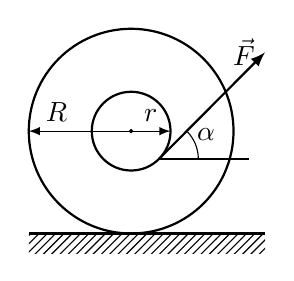
\begin{tikzpicture}
	\coordinate (A) at (3, 2.3);
    \coordinate (B) at (1.6533,0.9464);
    \coordinate (C) at (2.8, 0.9464);

	\draw [draw=none, pattern=north east lines] (3, 0) rectangle (0,-0.25);
	\draw [thick] (0,0) -- (3,0);
	\draw [fill] (1.3,1.3) circle (0.02);
	\draw [thick] (1.3,1.3) circle (0.5);
	\draw [thick] (1.3,1.3) circle (1.3);
	\draw [arrows={-latex}, thick] (1.6533,0.9464) -- (3, 2.3) node [above, left]  {$\vec{F}$};
	\draw (B) -- (C);
	\pic [draw, -, angle eccentricity=1.5] {angle = C--B--A};
	\node [right=17pt, above=3pt] at (B) {$\alpha$};
	\draw [arrows={-latex}] (1.3,1.3) -- (1.8, 1.3) node [above, midway]  {$r$};
	\draw [arrows={-latex}] (1.3,1.3) -- (0, 1.3) node [right=10pt, above]  {$R$};
\end{tikzpicture}
\end{document}